
%(BEGIN_QUESTION)
% Copyright 2015, Tony R. Kuphaldt, released under the Creative Commons Attribution License (v 1.0)
% This means you may do almost anything with this work of mine, so long as you give me proper credit

The direction of rotation for a three-phase AC electric motor may be reversed by swapping any two of the three power conductor connections.  With this in mind, explain how this reversing motor control circuit works:

$$\includegraphics[width=15.5cm]{i01391x01.eps}$$

In particular, what if the function of the two normally-closed ``M'' contacts (called {\it interlock} contacts) in the control circuit?  What do you think might happen if those contacts were not there?

\vskip 20pt \vbox{\hrule \hbox{\strut \vrule{} {\bf Suggestions for Socratic discussion} \vrule} \hrule}

\begin{itemize}
\item{} Explain {\it why} reversing any two phase conductors supplying AC power to an induction motor will cause it to reverse direction.
\item{} Explain what {\it arc flash} is, and how to protect yourself from it while working on high-voltage motor control circuits such as this one.
\item{} Suppose an electrician tries to force the motor to spin in its forward direction by connecting a temporary jumper wire across relay coil M1.  Will this accomplish the desired result?  Explain why or why not, and also identify any potential safety hazards in doing this.
\item{} Suppose an electrician tries to force the motor to spin in its forward direction by connecting a temporary jumper wire across the ``Forward'' pushbutton.  Will this accomplish the desired result?  Explain why or why not, and also identify any potential safety hazards in doing this.
\item{} Suppose an electrician tries to force the motor to spin in its forward direction by connecting three temporary jumper wires across the M1 contacts.  Will this accomplish the desired result?  Explain why or why not, and also identify any potential safety hazards in doing this.
\end{itemize}

\underbar{file i01391}
%(END_QUESTION)





%(BEGIN_ANSWER)

The normally-closed contacts are referred to as {\it interlock} contacts, and they prevent simultaneous {\it forward} and {\it reverse} actuation of the motor.
 
%(END_ANSWER)





%(BEGIN_NOTES)

Of course, if both forward and reverse contactors ever were to simultaneously energize, the result would be a direct phase-to-phase short-circuit!









\vfil \eject

\noindent
{\bf Summary Quiz:}

Explain in detail what function {\it interlock contacts} serve in a motor control circuit.   Feel free to use a practical example if it helps your explanation.

%INDEX% Final Control Elements, valve: electric actuator

%(END_NOTES)


